\documentclass{amsart}
\usepackage{amsmath}
\usepackage{amssymb}
\usepackage{amsthm}
%\usepackage{MnSymbol}
\usepackage{bm}
\usepackage{accents}
\usepackage{mathtools}
\usepackage{tikz}
\usetikzlibrary{calc}
\usetikzlibrary{decorations.pathmorphing,shapes}
\usetikzlibrary{automata,positioning}
\usepackage{tikz-cd}
\usepackage{forest}
\usepackage{braket} 
\usepackage{listings}
\usepackage{mdframed}
\usepackage{verbatim}
\usepackage{physics2}
\usephysicsmodule{ab,ab.legacy,diagmat,xmat}
\usepackage{derivative}
\usepackage{fixdif}
\usepackage{stmaryrd}
% \usepackage{euscript} 
% \usepackage[mathcal]{eucal}
\usepackage{stackengine} 
%\usepackage{/home/patrickl/homework/macaulay2}

%font
\usepackage[sc]{mathpazo}
\usepackage{inconsolata}
\usepackage{microtype}
% \usepackage{fontspec} 
% \setmainfont{Tex Gyre Pagella}
\usepackage[OT1,euler-digits]{eulervm}
% \usepackage{euler-math} 
\usepackage[scaled=0.86]{berasans}
% \let\sffamilyold\sffamily
% \def\sffamily{\fontencoding{T1}\sffamilyold}
% \setmonofont{Inconsolatazi4}

%CS packages
\usepackage{algorithmicx}
\usepackage{algpseudocode}
\usepackage{algorithm}

% typeset and bib
\usepackage[english]{babel} 
% \usepackage[utf8]{inputenc} 
% \usepackage[T1]{fontenc}
% \usepackage[backend=biber,style=alphabetic,maxalphanames=4,maxnames=5,hyperref]{biblatex}
\usepackage[bookmarks, colorlinks, breaklinks]{hyperref} 
\hypersetup{linkcolor=blue,citecolor=magenta,filecolor=black,urlcolor=blue}
\usepackage{cleveref}
\usepackage{graphicx}
\graphicspath{{./}}


% other formatting packages
\usepackage{float}
\usepackage{booktabs}
\usepackage[shortlabels]{enumitem}
\setitemize{noitemsep}
\usepackage{csquotes}
%\usepackage{titlesec}
%\usepackage{titling}
%\usepackage{fancyhdr}
%\usepackage{lastpage}
% \usepackage{parskip}
\newlist{mydescription}{description}{1}
\setlist[mydescription]{style=nextline,
                        font=\bfseries,
                        % Tweak the next 4 options as needed:
                        labelindent=1cm, 
                        leftmargin =2cm,
                        rightmargin=1cm,
                        topsep     =1ex
                       }

\usepackage{lipsum}

% delimiters
\DeclarePairedDelimiter{\gen}{\langle}{\rangle}
\DeclarePairedDelimiter{\floor}{\lfloor}{\rfloor}
\DeclarePairedDelimiter{\ceil}{\lceil}{\rceil}


\newtheorem{thm}{Theorem}[section]
\newtheorem{cor}[thm]{Corollary}
\newtheorem{prop}[thm]{Proposition}
\newtheorem{lem}[thm]{Lemma}
\newtheorem{conj}[thm]{Conjecture}
\newtheorem{quest}[thm]{Question}
\newtheorem{claim}[thm]{Claim}

\theoremstyle{definition}
\newtheorem{defn}[thm]{Definition}
\newtheorem{defns}[thm]{Definitions}
\newtheorem{con}[thm]{Construction}
\newtheorem{exm}[thm]{Example}
\newtheorem{exms}[thm]{Examples}
\newtheorem{notn}[thm]{Notation}
\newtheorem{notns}[thm]{Notations}
\newtheorem{addm}[thm]{Addendum}
\newtheorem{exer}[thm]{Exercise}

\theoremstyle{remark}
\newtheorem{rmk}[thm]{Remark}
\newtheorem{rmks}[thm]{Remarks}
\newtheorem{warn}[thm]{Warning}
\newtheorem{sch}[thm]{Scholium}


% unnumbered theorems
\theoremstyle{plain}
\newtheorem*{thm*}{Theorem}
\newtheorem*{prop*}{Proposition}
\newtheorem*{lem*}{Lemma}
\newtheorem*{cor*}{Corollary}
\newtheorem*{conj*}{Conjecture}

% unnumbered definitions
\theoremstyle{definition}
\newtheorem*{defn*}{Definition}
\newtheorem*{exer*}{Exercise}
\newtheorem*{defns*}{Definitions}
\newtheorem*{con*}{Construction}
\newtheorem*{exm*}{Example}
\newtheorem*{exms*}{Examples}
\newtheorem*{notn*}{Notation}
\newtheorem*{notns*}{Notations}
\newtheorem*{addm*}{Addendum}


\theoremstyle{remark}
\newtheorem*{rmk*}{Remark}

% shortcuts
\newcommand{\Ima}{\mathrm{Im}}
\newcommand{\A}{\mathbb{A}}
\newcommand{\G}{\mathbb{G}}
\newcommand{\N}{\mathbb{N}}
\newcommand{\R}{\mathbb{R}}
\newcommand{\C}{\mathbb{C}}
\newcommand{\Z}{\mathbb{Z}}
\newcommand{\Q}{\mathbb{Q}}
\newcommand{\E}{\mathbb{E}}
\renewcommand{\k}{\Bbbk}
\renewcommand{\L}{\mathbb{L}}
\renewcommand{\P}{\mathbb{P}}
\newcommand{\M}{\mathcal{M}}
\newcommand{\Mbar}{\overline{\mathcal{M}}}
\newcommand{\g}{\mathfrak{g}}
\newcommand{\h}{\mathfrak{h}}
\newcommand{\n}{\mathfrak{n}}
\renewcommand{\b}{\mathfrak{b}}
\newcommand{\ep}{\varepsilon}
\newcommand*{\dt}[1]{%
   \accentset{\mbox{\Huge\bfseries .}}{#1}}
%\renewcommand{\abstractname}{Official Description}
\newcommand{\mc}[1]{\mathcal{#1}}
% \newcommand{\msc}[1]{\mathscr{#1}}
\newcommand{\T}{\mathbb{T}}
\newcommand{\mf}[1]{\mathfrak{#1}}
\newcommand{\mbf}[1]{\mathbf{#1}}
\newcommand{\bv}{\mbf{v}}
\newcommand{\bq}{\mbf{q}}
\newcommand{\bp}{\mbf{p}}
\newcommand{\btau}{\bm{\tau}}
\newcommand{\mr}[1]{\mathrm{#1}}
\newcommand{\on}[1]{\operatorname{#1}}
\newcommand{\ms}[1]{\mathsf{#1}}
\newcommand{\mt}[1]{\mathtt{#1}}
\newcommand{\ol}[1]{\overline{#1}}
\newcommand{\ul}[1]{\underline{#1}}
\newcommand{\wt}[1]{\widetilde{#1}}
\newcommand{\wh}[1]{\widehat{#1}}
\renewcommand{\div}{\operatorname{div}}
\newcommand{\1}{\mathbf{1}}
\newcommand{\2}{\mathbf{2}}
\newcommand{\3}{\mathbf{3}}
\newcommand{\I}{\mathrm{I}}
\newcommand{\II}{\mr{I}\hspace{-1.3pt}\mr{I}}
\newcommand{\III}{\mr{I}\hspace{-1.3pt}\mr{I}\hspace{-1.3pt}\mr{I}}
\renewcommand{\v}{\mbf{v}}
\newcommand{\w}{\mbf{w}}
\newcommand{\bmu}{\bm{\mu}}
\newcommand{\pre}{\mr{pre}}
\newcommand{\vir}{\mr{vir}}
\newcommand{\fl}{\mr{fl}}
\newcommand{\ps}[1]{\llbracket #1 \rrbracket}
\newcommand{\ls}[1]{\llparenthesis #1 \rrparenthesis}

\DeclareMathOperator{\Der}{Der}
\DeclareMathOperator{\Tor}{Tor}
\DeclareMathOperator{\Hom}{Hom}
\DeclareMathOperator{\End}{End}
\DeclareMathOperator{\Ext}{Ext}
\DeclareMathOperator{\ad}{ad}
\DeclareMathOperator{\Aut}{Aut}
\DeclareMathOperator{\Rad}{Rad}
\DeclareMathOperator{\Pic}{Pic}
\DeclareMathOperator{\NS}{NS}
\DeclareMathOperator{\supp}{supp}
\DeclareMathOperator{\Supp}{Supp}
\DeclareMathOperator{\depth}{depth}
\DeclareMathOperator{\sgn}{sgn}
\DeclareMathOperator{\spec}{Spec}
\DeclareMathOperator{\Spec}{Spec}
\DeclareMathOperator{\proj}{Proj}
\DeclareMathOperator{\Proj}{Proj}
\DeclareMathOperator{\ord}{ord}
\DeclareMathOperator{\Div}{Div}
\DeclareMathOperator{\Bl}{Bl}
\DeclareMathOperator{\coker}{coker}
\DeclareMathOperator{\ev}{ev}
\DeclareMathOperator{\st}{st}
\DeclareMathOperator{\pr}{pr}
\DeclareMathOperator{\ch}{ch}
\DeclareMathOperator{\Cont}{Cont}

% \addbibresource{../../notes/math.bib}

\title[Axiomatic enumerative geometry]{Axiomatic approach to enumerative geometry: Lagrangian cone, CohFTs, and R-matrix actions}
\author{Patrick Lei}
\date{January 6, 2025}
\allowdisplaybreaks

\begin{document}
    
\begin{abstract}
    In these two lectures, I will explain an axiomatic approach to Gromov-Witten type enumerative theories constructed by Kontsevich-Manin, Givental, and others. A key insight is that there is an action of the symplectic loop group on CohFTs such that the effect on generating functions is given by geometric quantization of symplectic matrices, which can be computed combinatorially as a sum over stable graphs.
\end{abstract}

\maketitle

\tableofcontents

\section{Moduli of curves and CohFTs}%
\label{sec:Moduli of curves and CohFTs}

We will denote by $\Mbar_{g,n}$ the moduli space of stable curves of genus $g$ with $n$ marked points. This is nonempty if and only if $2g-2+n > 0$, in which case it is a Deligne-Mumford stack of dimension $3g-3+n$. There is a combinatorial structure to the collection of $\Mbar_{g,n}$, which is given by a collection of morphisms.
\begin{itemize}
    \item There is the gluing morphism 
        \[q \colon \Mbar_{g,n+1} \times \Mbar_{h, m+1} \to \Mbar_{g+h,n+m}, \] 
        which takes two curves and glues them along the last marked point to form a node;
    \item There is the self-gluing morphism \[s \colon \Mbar_{g-1,n+2} \to \Mbar_{g,n},\] 
        which glues the last two marked points.
\end{itemize}
There is of course another interesting map, which is the forgetful map
\[ \pr \colon \Mbar_{g,n+1} \to \Mbar_{g,n} \]
given by deleting the last marked point and then stabilizing. We are now able to define our enumerative theories of interest, which include Gromov-Witten theory.

\begin{defn}
    Given a vector space $V$ with a nondegenerate symmetric bilinear form $\eta$ and a unit element $\1 \in V$, a \textit{Cohomological Field Theory (CohFT)} $\Omega$ on $V$ is a collection $\Omega_{g,n}$ of $S_n$-equivariant linear maps
    \[ \Omega_{g,n} \colon V^{\otimes n} \to H^*(\Mbar_{g,n}) \]
    which satisfy the basic identity
    \[ \Omega_{0,3}(\1, u,v) = \eta(u,v) \]
    and the following combinatorial identities (we will let $e_{\mu}$ be a basis of $V$ such that $e_1 = \1$ and $e^{\mu}$ be the dual basis):
    \begin{align*}
        q^* \Omega_{g+h,n+m}(\bv_1, \bv_2) &= \sum_{\mu} \Omega_{g,n+1}(\bv_1, e_{\mu}) \cdot \Omega_{h,m+1}(  \bv_2, e^{\mu} ); \\
        s^* \Omega_{g,n}(\bv) &= \sum_{\mu} \Omega_{g,n+2}(\bv, e_{\mu}, e^{\mu}).
    \end{align*}
    If in addition the identity
    \[ \pr^*\Omega_{g,n}(\bv) = \Omega_{g,n+1}(\bv,\1) \]
    is satisfied, then we say the CohFT has a \textit{flat unit} (or satisfies the \textit{string equation}).
\end{defn}
All of this can be generalized to super vector spaces, but for simplicity we will not deal with this case.

\begin{exm}
    The most important example of a CohFT is the Gromov-Witten theory of a smooth projective variety $X$. Here, recall that the source of a stable map is a \textbf{prestable} curve, so there is a stabilization morphism
    \[ \st \colon \Mbar_{g,n}(X,\beta) \to \Mbar_{g,n} \]
    which forgets the map and stabilizes the curve. Then, working over the Novikov ring, we will set $V = H^*(X)$, $\eta$ to be the Poincar\'e pairing, and $\1$ to be the fundamental class of $X$. The linear maps $\Omega^X_{g,n}$ are given by the formulae
    \[ \Omega_{g,n}^X(\btau) \coloneqq \sum_{\beta} q^{\beta} \st_* \ab(\prod_{i=1}^n \ev_i(\tau_i) \cap [\Mbar_{g,n}(X,\beta)]^{\vir}), \]
    where $\ev_i \colon \Mbar_{g,n}(X,\beta) \to X$ is the $i$-th evaluation map.
\end{exm}

\begin{exm}
    Let $\pi \colon \mc{C}_{g,n} \to \Mbar_{g,n}$ be the universal curve. Then the \textit{Hodge bundle} is the vector bundle 
    \[ \E_{g,n} \coloneqq \pi_* \omega_{\pi}. \]
    We then consider the vector space $V = \C$ with the usual pairing and define the CohFT $\Omega^{\E}$ by the formula
    \[ \Omega^{\E}_{g,n} \coloneqq c(\E_{g,n}). \]
    The gluing axioms are satisfied by the equation $q^* \E_{g+h} = \E_g \oplus \E_h$ and the exact sequence
    \[ 0 \to \E_{g-1} \to \E_g \to \mc{O} \to 0. \]
    Here, because genus zero components do not contribute to global sections of $\omega$ and $\E$ does not depend on the marked points, this CohFT has a flat unit.
\end{exm}

\begin{rmk}
    We will see later that this is related to the GW CohFT of a point by the quantum Riemann-Roch theorem. 
\end{rmk}

Given a CohFT $\Omega$, we may produce invariants by pairing the classes $\Omega_{g,n}(\bv)$ with various cohomology classes on $\Mbar_{g,n}$. The most important ones to consider are the classes
\[ \bar{\psi}_i \coloneqq c_1( s_i^* \omega_{\pi} ), \]
where $s_i \colon \Mbar_{g,n} \to \mc{C}_{g,n}$ is the $i$-th marked point.

\begin{rmk}
    In Gromov-Witten theory, these are called \textit{ancestors}. There are also descendants, which are given by the same formula except using the moduli space $\mf{M}_{g,n}$ of prestable curves instead of $\Mbar_{g,n}$, where we factor the morphism $\st$ defined above as
    \[ \Mbar_{g,n}(X,\beta) \xrightarrow{\text{forget map}} \mf{M}_{g,n} \xrightarrow{\text{stabilize}} \Mbar_{g,n}. \]
    The descendant classes are denoted by $\psi_i$.
\end{rmk}

\begin{exm}
    We will calculate an invariant which will appear in the GW theory of Calabi-Yau threefolds. For any CohFT $\Omega$, consider the invariant
    \[ \ab<\1\bar{\psi}_1>_{1,1}^{\Omega}\coloneqq \int_{\Mbar_{1,1}} \Omega_{1,1}(\1)\bar{\psi}_1. \]
    Using the second gluing equation, the degree zero part of $\Omega_{1,1}(\1)$ is equal to
    \[ \sum_{\mu} \Omega_{g,n+2}(\1, e_{\mu}, e^{\mu}) = \sum_{\mu} \eta(e_{\mu}, e^{\mu}), \]
    which yields the (graded) dimension $\chi(V)$ of $V$. Therefore, we obtain
    \[ \ab<\1\bar{\psi}_1>_{1,1}^{\Omega} = \frac{\chi(V)}{24}. \]
\end{exm}

\begin{exm}
    Consider the GW CohFT of a point. This is given by $V = \C$ with the usual pairing and the formula 
    \[ \Omega_{g,n} = 1. \]
    Then we define the invariants
    \[ \ab<\bar{\psi}_1^{a_1} \cdots \bar{\psi}_n^{a_n}>_{g,n} \coloneqq \int_{\Mbar_{g,n}} \Omega_{g,n} \cdot \bar{\psi}_1^{a_1} \cdots \bar{\psi}_n^{a_n}. \]
    \begin{thm}[Kontsevich]
        The function
        \[ \mc{D} \coloneqq \exp \ab(\sum_{g,n} \frac{\hbar^{g-1}}{n!}\sum_{a_1 + \cdots + a_n = n} \ab<\bar{\psi}_1^{a_1} \cdots \bar{\psi}_n^{a_n}>_{g,n} t_{a_1}\cdots t_{a_n}) \]
        is annihilated by the operators
        \begin{align*}
            L_{-1} \coloneqq{}& -\pdv{}{t_0} + \frac{\hbar^{-1}}{2} t_0^2 + \sum_{i=0}^{\infty} t_{i+1} \pdv{}{t_i};\\
            L_0 \coloneqq{}& -\frac{3}{2} \pdv{}{t_1} + \sum_{i=0}^{\infty} \frac{2i+1}{2} t_i \pdv{}{t_i} + \frac{1}{16};\\
            L_n \coloneqq{}& -\frac{(2n+3)!!}{2^{n+1}} \pdv{}{t_{n+1}} + \sum_{i=0}^{\infty} \frac{(2i+2n+1)!!}{(2i-1)!! 2^{n+1}} t_i \pdv{}{t_{i+n}} \\
            &+ \frac{\hbar}{2} \sum_{i=0}^{n-1} \frac{(2i+1) (2i-1) \cdots (2i+1-2n)}{2^{n+1}} \pdv{}{t_i,t_{n-1-i}}.
        \end{align*}
    \end{thm}
\end{exm}

\begin{rmk}
    This result (Virasoro constraints for a point) is equivalent to $\mc{D}$ being a tau-function for the KdV hierarchy and has been generalized by various authors.
\end{rmk}

\section{The genus-zero picture}%
\label{sec:The genus-zero picture}

A CohFT in genus zero defines a Frobenius manifold. In particular, there is a product structure defined by the formula
\[ \eta(\tau_1 \star_{\tau} \tau_2, \tau_3) \coloneqq \sum_n \frac{1}{n!} p_* \ab<\tau_1, \tau_2, \tau_3, \tau,\ldots, \tau>_{0,3+n}^{\Omega} \]
and the quantum connection, which is defined by the formula
\[ \nabla_{\mu} \coloneqq \partial_{e_{\mu}} + \frac{1}{z} e_{\mu} \star_{\tau}. \]
The structure of a Frobenius manifold comes from a function $\mc{F}_0$, which is known as the \textit{genus-zero descendant potential} and satisfies a set of PDEs, which are the string equation, dilaton equation, and an infinite set of topological recursion relations, where we write $\bv = \sum_{\mu,n} t^{\mu}_n e_{\mu} z^n \in V\ps{z}$:
\begin{align*}
    \pdv{}{t_0^1} \mc{F}_0 &= \frac{1}{2} (\bv_0, \bv_0) + \sum_{n=0}^{\infty} \sum_{\mu} t_{n+1}^{\mu} \pdv{}{t_n^{\mu}} \mc{F}_0; \\
    \pdv{}{t_1^1} \mc{F}_0 &= \sum_{n=0}^{\infty} \sum_{\mu} t_n^{\mu} \pdv{}{t_n^{\mu}}\mc{F}_0 - 2 \mc{F}_0; \\
    \pdv{}{t_{k+1}^{\alpha},t_m^{\beta},t_n^{\gamma}} \mc{F}_0 &= \sum_{\mu,\nu} \pdv{}{t_k^{\alpha},t_0^{\mu}} \mc{F}_0 \cdot \eta^{\mu\nu} \cdot \pdv{}{t_0^{\nu},t_{m}^{\beta},t_n^{\gamma}} \mc{F}_0.
\end{align*}
To state the following result, we consider the infinite-dimensional vector space $V\ls{z^{-1}}$ (or a completion of this) with the symplectic form
\[ (\mbf{f}(z), \mbf{g}(z)) \coloneqq \on{Res}_{z=0}\eta(\mbf{f}(-z), \mbf{g}(z)). \]
We also consider the new variable\footnote{This is called the \textit{dilaton shift}.} $\bq = \bv - z$, so $\mc{F}_0$ is now a function near $\bq = -z$.

\begin{thm}[Givental]
    $\mc{F}$ satisfies the above PDEs if and only if the graph $\mc{L}$ of $\d{\mc{F}}$ is a Lagrangian cone with vertex at $\bq = 0$ such that its tangent spaces $L$ are tangent to $\mc{L}$ exactly along $zL \subset L$.
\end{thm}

We may recover the Lagrangian cone $\mc{L}$ by the following procedure. We find a fundamental solution 
\[ S = \mr{Id} + S_1 z^{-1} + S_2 z^{-2} + \cdots \]
to the quantum connection, which satisfies the equation
\[ z \pdv{}{t^{\mu}}S = e_{\mu} \star S. \]
Then, setting $J \coloneqq z S^*(z) \1$, we can then recover the Lagrangian cone by the following procedure:
\begin{itemize}
    \item The derivatives $\pdv{}{t^{\mu}} J$ form a basis of $L \cap V\ps{z^{-1}}$;
    \item This implies that $z \pdv{}{t^{\mu},t^{\nu}} \in L \cap V \ps{z^{-1}}$. Writing these in terms of the first derivatives and using the fact that $J$ solves the quantum connection, we recover the Frobenius structure and hence the Lagrangian cone.
\end{itemize}

In Gromov-Witten theory, there is an explicit formula for the fundamental solution in terms of descendant invariants. It is given by
\[ S_{\tau}(z) \phi \coloneqq \phi + \sum_{\mu} \sum_{n,\beta} \frac{q^{\beta}}{n!} e^{\mu} \ab<\frac{e_{\mu}}{z-\psi_1}, \phi, \tau, \ldots, \tau>_{0,n+2,\beta}^{X}. \]

\begin{exm}
    Let $X$ be the quintic threefold. We will use the genus-zero mirror theorem of Givental to compute the quantum product on $H^*(X)$. Let
    \begin{align*}
        I(q,z) &\coloneqq z \sum_{d \geq 0} q^d \frac{\prod_{m=1}^{5d} (5H+mz)}{\prod_{m=1}^d (H+mz)^5}  \\
        &= z I_0(q) + I_1(q) \cdot H + I_2(q) \cdot \frac{H^2}{z} + I_3(q) \cdot \frac{H^3}{z^2}
    \end{align*}
    be the (very small) $I$-function of $X$. Setting $Q(q) \coloneqq q e^{\frac{I_1(q)}{I_0(q)}}$, the mirror theorem states that
    \[ J(0,Q(q),z) = \frac{I(q,z)}{I_0(q)}. \]
    Because the mirror map $q \mapsto Q(q)$ corresponds to setting $\tau = \frac{I_1(q)}{I_0(q)} H$ by the divisor equation, we can use the mirror theorem to compute $\star_{\tau}$. Because of our nonstandard choice of the $I$-function, the quantum connection becomes the ODE
    \[ (H+zD) S_{\tau}(z)^* = S_{\tau}(z)^* \cdot I_{11} H \star_{\tau}, \]
    where $D \coloneqq q \odv{}{q}$ (here, the coordinate is $\log q$) and $I_{11} \coloneqq 1 + D \ab(\frac{I_1(q)}{I_0(q)})$. An explicit computation using the mirror theorem and the results of Zagier-Zinger yields
    \begin{align*}
        I_{11} H + \cdots &= S_{\tau}(z)^* (I_{11} H \star_{\tau} \1) \\
        \ab( 1 + D\ab(\frac{\frac{I_1}{I_0} + D \ab(\frac{I_2}{I_0})}{I_{11}}) ) H^2 + \cdots &= S_{\tau}(z)^* (I_{11} H \star_{\tau} H) \\
        I_{11} H^3 &= S_{\tau}(z)^* (I_{11}H \star_{\tau} H^2).
    \end{align*}
    Because $S_{\tau}$ begins with the identity, this computes $H \star_{\tau}$.
\end{exm}


\section{$R$-matrix action}%
\label{sec:R-matrix action}

In the early 2000s, Givental discovered a remarkable property of axiomatic enumerative theories, namely that one can transform CohFTs by the action of matrices $R(z) = R_0 + R_1 z + R_2 z^2 + \cdots \in \Hom(V, V')\ps{z}$ which satisfy the property
\[ R^*(-z) R(z) = \mr{Id}_V. \]
Traditionally, the literature requires that $V = V'$ and $R_0 = \mr{Id}$, but the MSP group has removed this restriction and also allows $\dim V < \dim V'$.

In order to define the action of $R$ on a CohFT $\Omega$ defined on $V$, we need to review some of the combinatorial structure of $\Mbar_{g,n}$. For a curve $C\in \Mbar_{g,n}(\C)$, we may consider the dual graph of $C$, which has vertices, edges, and legs, which are defined as follows:
\begin{itemize}
    \item The vertices correspond to irreducible components of $C$ and are labelled by a non-negative integer, which is the genus;
    \item The edges correspond to nodes of $C$ (in particular, we allow loops);
    \item The legs correspond to marked points.
\end{itemize}
Any graph which appears as the dual graph of a stable curve is called a \textit{stable graph}.

\begin{figure}[htpb]
  \centering
  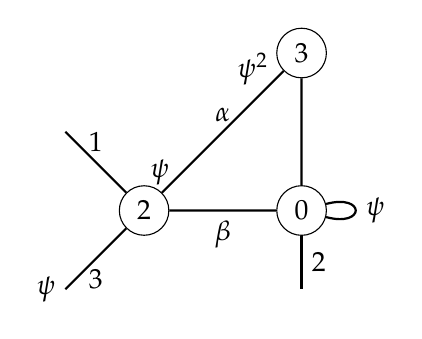
\begin{tikzpicture}[scale=1,transform shape,every loop/.style={}]
    \node[circle,draw] (A) at (0,0) {$2$};
    \node[circle,draw] (B) at (2,2) {$3$};
    \node[circle,draw] (C) at (2,0) {$0$};
    \draw[thick] (A) -- node[above]{$\alpha$} (B) -- (C) -- node[below]{$\beta$} (A);
    \draw[thick] (A) -- node[below]{$3$} (-1,-1);
    \draw[thick] (A) -- node[above]{$1$} (-1,1);
    \draw[thick] (C) -- node[right]{$2$} (2,-1);
    \draw[thick] (C) edge[loop right] node[right] {$\psi$} (C);
    \node[anchor=east] at (-1,-1) {$\psi$};
    \node[anchor=east] at (1.7,1.8) {$\psi^2$};
    \node[anchor=south] at (0.2,0.2) {$\psi$};
  \end{tikzpicture}
  \caption{Example of a stable graph in $\ol{\mc{M}}_{7,3}$ and associated tautological class. This stable graph describes the image of a map
    $\ol{\mc{M}}_{2,4} \times \ol{\mc{M}}_{3,2} \times \ol{\mc{M}}_{0,5} \to \ol{\mc{M}}_{7,3}$.}
  \label{fig:stablegraph}
\end{figure}

The first type of action on CohFTs is a translation action. Let $T \in V\ps{z}$. For a CohFT $\Omega$, we define
\[ (T\Omega)_{g,n}(\bv) \coloneqq \sum_m \frac{1}{m!} p_* \Omega_{g,n+m}(\bv, T,\ldots,T) \]
whenever the infinite sum makes sense.

\begin{exm}
    If $\Omega^X$ is the GW CohFT of a smooth projective variety $X$ and $\tau \in H^2(X)$ is a divisor class, then the infinite sum makes sense and we can define the shifted GW CohFT $\Omega^{X,\tau}$ of $X$. For example, if $X$ is the quintic threefold and $\tau = \frac{I_1}{I_0} H$, then shifting to $\tau$ is the same as the mirror map $q \mapsto Q(q) = q e^{\frac{I_1}{I_0}}$.
\end{exm}

The second type of action is the action of a matrix $R$ as in the beginning of this section. Let $G_{g,n}$ define the set of all stable graphs of genus $g$ with $n$ legs. Then we define
\[ (R\Omega)_{g,n} \coloneqq \sum_{\Gamma \in G_{g,n}} \frac{1}{\ab|\Aut \Gamma|} \on{Cont}_{\Gamma}, \]
where $\on{Cont}_{\Gamma}$ is defined by the following construction:
\begin{itemize}
    \item At the $i$-th leg, we place the map 
        \[ R(-\bar{\psi}_i)^* \in \Hom(V',V) \ps{\bar{\psi}_i}; \]
    \item At every edge, we place the bivector
        \[ V(\bar{\psi}_1, \bar{\psi}_2) \coloneqq \sum_{\mu} \frac{e_{\mu} \otimes e^{\mu} - R(-\bar{\psi}_1)^* e_{\mu} \otimes R(-\bar{\psi}_2)^* e^{\mu}}{\bar{\psi}_1 + \bar{\psi}_2}; \]
    \item At every vertex, we place the linear map
        \[ \Omega_{g_v, n_v} \colon V^{\otimes n_v} \to H^*(\Mbar_{g_v, n_v}); \]
    \item Finally, we consider the pushforward in cohomology along the gluing morphism $\prod_v \Mbar_{g_v, n_v} \to \Mbar_{g,n}$.
\end{itemize}

\begin{defn}
    Let $R$ be as above. Then we define the translation
    \[ T_R \coloneqq z (\1 - R(-z)^* \1') \in z V'\ps{z}. \]
    Whenever it makes sense, we define
    \[ R.\Omega \coloneqq RT\Omega. \]
\end{defn}

\begin{thm}[Chang-Guo-Li]
    Suppose we work with coefficients in $\C\ps{q}$. Then if
    \[ T_R \in z^2 V \ps{z} + zq V \ps{z}, \]
    $R.\Omega$ is a well-defined CohFT. Moreover, if $\dim V = \dim V'$, $\1'$ is a unit for $R.\Omega$.
\end{thm}

We would like to remark a bit more about the translation action when $R_0 \neq \mr{Id}$. For simplicity, we will assume that $V = V'$ and $R_0 \1 = c \cdot \1$ for some constant $c$. Then we set $\tilde{T}_R \coloneqq z( \1 - c R(z)^{-1} \1)$ and use the dilaton equation to compute
\begin{align*}
    T_R \Omega_{g,n}(\bv) &= \sum_{m=0}^{\infty} \frac{1}{m!} p_*\Omega_{g,n+m}(\bv, T_R, \ldots, T_R) \\
    &= \sum_{k,\ell \geq 0} \frac{1}{k!\ell!} p_* \Omega_{g,n+k+\ell}(\bv, ( (1-c^{-1})\1 \cdot \psi )^{\otimes k}, ( c^{-1} \tilde{T}_R )^{\otimes \ell}) \\
    &= \sum_{k,\ell \geq 0} \frac{(1-c^{-1})^k \cdot c^{-\ell}}{\ell!} \binom{2g-2+n+k+\ell-1}{k} p_* \Omega_{g,n+\ell}(\bv, \tilde{T}_R^{\otimes \ell}) \\
    &= \sum_{m=0}^{\infty} \frac{c^{2g-2+n}}{m!} p_* \Omega_{g,n+m}(\bv, \tilde{T}_R, \ldots, \tilde{T}_R)
\end{align*}
whenever this makes sense.


\section{Reconstruction theorem}%
\label{sec:Reconstruction theorem}

Recall that every CohFT defines a Frobenius algebra. We will call a CohFT \textit{semisimple} if the corresponding Frobenius algebra is semisimple.

\begin{thm}[Teleman]
    Let $\Omega$ be a semisimple CohFT with flat unit and $\omega$ be its topological part. If $\Omega$ is semisimple, there exists a unique 
    \[ R = \mr{Id} + R_1 z + \cdots \in \End(V)\ps{z} \]
    such that
    \[ \Omega = R.\omega. \]
\end{thm}

\begin{exm}
    Recall the Hodge bundle CohFT from before. Recall that it is given by the formula
    \[ \Omega^{\E}_{g,n} = c(\E) = 1 + \lambda_1 + \cdots + \lambda_g. \]
    Taking the degree zero part, we see that $\omega^{\E}$ is the GW CohFT of a point. Using Mumford's computation
    \[ \ch(\E) = g + \sum_{k=1}^{\infty} \frac{B_{2k}}{(2k)!}\ab(\kappa_{2k-1} + \frac{1}{2}\iota_*\sum_{i=0}^{2k-2} \bar{\psi}_1^{i} \bar{\psi}_2^{2g-2+i}), \]
    where $\kappa_{m} = p_* \bar{\psi}_{n+1}^{m+1}$, $B_{2k}$ are the Bernoulli numbers, and $\iota$ is the inclusion of the boundary up to a $2:1$ \'etale cover, and the formula
    \[ c(E) = \exp \ab(-\sum_k (-1)^k (k-1)!\ch_k(E)) \]
    for any vector bundle $E$ (or by just using the quantum Riemann-Roch theorem\footnote{There is a sign error in Coates-Givental, which has propagated to the rest of the literature.} directly), we obtain the $R$-matrix
    \[ R(z) = \exp\ab( \sum_{k=1}^{\infty} \frac{B_{2k}}{2k(2k-1)} z^{2k-1}) = 1+\frac{1}{12}z + \cdots. \]

    As a sanity check, we will compute $\Omega_{1,1}^{\E}$ using the $R$-matrix. First, we consider the stable graphs in~\Cref{fig:03graphloop}.
    \begin{figure}[htpb]
    \begin{center}
    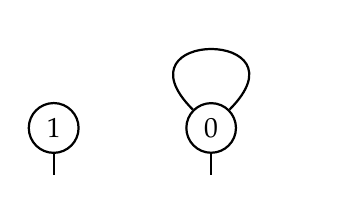
\begin{tikzpicture}[scale=1, transform shape, every loop/.style={}]
    \node[circle,draw=black,thick] (B) at (-1,0) {$1$};
    \draw[-,thick] (B) -- (-1,-0.6);
    \node[circle,draw=black,thick] (A) at (1,0) {$0$};
    \draw[-,thick] (A) -- (1,-0.6);
    \path[every node/.style={font=\sffamily\small},thick]
        (A)   edge[loop] (A);
    \end{tikzpicture}
    \end{center}
    \caption{Stable graphs for $g=1, n=1$}%
    \label{fig:03graphloop}
    \end{figure}
    The first graph $\Gamma_1$ gives us the contribution
    \begin{align*}
        \Cont_{\Gamma_1} &= T\omega_{1,1}^{\E}(R(z)^{-1}\1) \\
        &= \omega_{1,1}^{\E}(R(z)^{-1}\1) + p_* \omega_{1,1}^{\E}(R(z)^{-1}\1, T_R(z)).
    \end{align*}
    Using the formula $B_2 = \frac{1}{6}$ and the fact that $\dim \Mbar_{1,1} = 1$, this becomes
    \[ 1 - \frac{1}{12}\psi_1 + \frac{1}{12} \kappa_1. \]
    The second graph does not receive tail contributions because $\dim \Mbar_{0,3} = 0$. The constant term of the edge contribution is $\frac{1}{12}$, so considering the automorphism and pushing forward to $\Mbar_{1,1}$ gives us
    \[ \Cont_{\Gamma_2} = \frac{1}{12} \Delta, \]
    where $\Delta$ denotes the boundary divisor (with the correct stack structure). Because $\psi_1 = \kappa_1$ in this case, we obtain
    \[ 1+\lambda_1 = 1 + \frac{1}{12}(\kappa_1 - \psi_1 + \Delta) = 1 + \frac{1}{12} \Delta. \]
\end{exm}

\section{Operator formalism and geometric quantization}%
\label{sec:Operator formalism and geometric quantization}

We will return to the symplectic formalism of Givental. This is more convenient for certain computations, but it is in fact equal to what we have before, at least when we want to calculate generating functions. Recall that we had a Frobenius manifold structure on $V$ and we considered the vector space $\mc{V}\coloneqq V\ls{z^{-1}}$ with symplectic form
\[ (\mbf{f}(z), \mbf{g}(z)) \coloneqq \on{Res}_{z=0} \eta(\mbf{f}(-z), \mbf{g}(z)). \]
If we consider the polarization given by $\mc{V}_+ = V[z]$ and $\mc{V}_- = z^{-1}V\ps{z^{-1}}$, then letting $\bq$ be as before (with the dilaton shift), let $\bp$ be coordinates on $\mc{V}_-$ such that $(\bq, \bp)$ form a system of Darboux coordinates for $\mc{V}$.

\begin{defn}
    We will call any formal function of the form
    \[ \mc{D} = \exp\ab(\sum_{g=0}^{\infty} \hbar^{g-1} \mc{F}_g) \]
    an \textit{asymptotic element of the Fock space}.
\end{defn}

Then given such an asymptotic element of the Fock space, we will quantize (infinitesimal) symplectic transformations on $\mc{V}$ by the following formulae:
\[ \wh{p_a p_b} \coloneqq \hbar \partial_{q_a} \partial_{q_b}, \qquad \wh{p_a q_b} \coloneqq q_b \partial_{q_a}, \qquad \wh{q_a q_b} = \frac{q_a q_b}{\hbar}. \]
In particular, this will allow us to understand expressions like $\hat{R} \mc{D}$. However, we need to be careful because our formulae will involve both the fundamental solution $S_{\tau}$ and the $R$-matrix, and $S_{\tau}$ is a power series in $z^{-1}$.\footnote{This is because we expand $\frac{1}{z-\psi} = \sum_{n=0}^{\infty} \psi^n z^{-n-1}$.}

\begin{thm}[Givental]
    An operator of the form $S(z^{-1}) = \mr{Id} + S_1 z^{-1} + \cdots$ acts on (asymptotic) elements of the Fock space by the formula
    \[ \hat{S}^{-1} \mc{D}(\bq) = e^{\frac{1}{2\hbar}W(\bq,\bq)} \mc{D}([S \bq]_+), \]
    where $W = \sum \eta(W_{mn}q_m, q_n)$ is defined by the formula
    \[ \frac{S(w^{-1})^* S(z^{-1}) - \mr{Id}}{w^{-1}+z^{-1}} = \sum \frac{W_{mn}}{w^m z^n}. \]
    Operators of the form $R(z) = \mr{Id} + R_1 z + \cdots$ act by the formula
    \[ \hat{R}\mc{D}(\bq) = e^{\frac{\hbar}{2} V(\partial_{\bq}, \partial_{\bq})} \mc{D}(R^{-1} \bq), \]
    where $V = \sum \eta(p_m, V_{mn} p_n)$ is defined by 
    \[ \frac{R(w)^* R(z) - \mr{Id}}{w+z} = \sum V_{mn} w^m z^n. \]
\end{thm}

For a semisimple CohFT, there is a system of \textit{canonical coordinates} $u_{\alpha}$ such that the $1$-form $\d{u}$ is a homomorphism of algebras $T_v V \to \C$. Then near a semisimple point, there is a asymptotic solution to the quantum connection of the form
\[ \Psi \cdot  R \cdot e^{\frac{U}{z}}, \]
where $\Psi$ switches from flat coordinates to canonical coordinates and $U = \on{diag}(u_{\alpha})$ is the matrix of canonical coordinates. Finally, define
\[ C = \frac{1}{2} \int^u \sum R_1^{\alpha\alpha} \d{u_{\alpha}}. \]
A corollary of Teleman's reconstruction theorem is the formula
\[ \mc{D}^X = e^{C(u)} \hat{S}^{-1}_{\tau} \hat{\Psi} \hat{R} \wh{e^{\frac{U}{z}}} \prod_{i=1}^{\dim V} \mc{D}^{\mr{pt}} \]
for the Gromov-Witten theory of any smooth projective variety with semisimple quantum cohomology.

\begin{exm}
    As a final example, we will apply Teleman's theorem to compute $F_1$ of any semisimple CohFT. Let $e_{\mu}$ denote an idempotent basis for the quantum product. We will compute
    \[ \int_{\Mbar_{1,1}} \Omega_{1,1}(e_{\beta}). \]
    Using the reconstruction theorem, we obtain
    \begin{align*}
        \int_{\Mbar_{1,1}}\Omega_{1,1}(e_{\beta}) ={}& \int_{\Mbar_{1,1}} T_R \omega_{1,1}(R(\bar{\psi})^{-1} e_{\beta}) + \frac{1}{2} T_R \omega_{0,3}(R(\bar{\psi})^{-1} e_{\beta}, V(\bar{\psi}_2, \bar{\psi}_3)) \\
        ={}& \int_{\Mbar_{1,1}}T_R\omega_{1,1}(e_{\beta}) - \int_{\Mbar_{1,1}} T_R \omega_{1,1}(R_1 e_{\beta})\bar{\psi} \\ 
        &+ \frac{1}{2}\sum_{\mu}  \omega_{0,3}(e_{\beta}, R_1 e^{\mu}, e_{\mu}) \\
        ={}& \int_{\Mbar_{1,1}} ( \omega_{1,1}(e_{\beta}) + p_* ( \omega_{1,2}(e_{\beta}, R_1 \1) \bar{\psi}_2^2 )) \\
        &- \int_{\Mbar_{1,1}} (\omega_{1,1}(R_1 e_{\beta})\bar{\psi}_1 + p_* ( \omega_{1,2}(R_1 e_{\beta}) \bar{\psi}_2^2 ) \bar{\psi}_1) \\
        &+ \frac{1}{2} \sum_{\mu} \eta(e_{\beta} \star e_{\mu}, R_1 e^{\mu}) \\
        ={}& \frac{1}{24} \sum_{\mu} ( \omega_{0,4}(e_{\mu}, e^{\mu}, e_{\beta}, R_1 \1) -\omega_{0,3}(e_{\mu}, e^{\mu}, R_1 e_{\beta}) )\\
        &+ \frac{1}{2} \eta(e_{\beta}, R_1 e^{\beta}) \\
        ={}& \frac{1}{24} \sum_{\mu}\sum_{\nu} \omega_{0,3}(e_{\mu}, e^{\mu}, e_{\nu})\omega_{0,3}(e^{\nu}, e_{\beta}, R_1 \1) \\
        &-\frac{1}{24} \sum_{\mu} \omega_{0,3}(e_{\mu}, e^{\mu}, R_1 e_{\beta}) + \frac{1}{2} (R_1)_{\beta\beta} \\
        ={}& \frac{1}{24} \ab(\eta(e^{\beta}, R_1 \1) - \sum_{\mu} \eta(e^{\mu}, R_1 e_{\beta})) + \frac{1}{2} (R_1)_{\beta\beta}.
    \end{align*}
    Using the identities
    \begin{align*}
        \eta(R_1 \1, e^{\beta}) - \sum_{\mu} \eta(R_1 e_{\beta}, e^{\mu}) &= \sum_{\mu} \Delta_{\mu} \int_{\Mbar_{0,4}} \Omega_{0,4}(e_{\mu}, e_{\mu}, e_{\mu}, e_{\beta}) \\
        &= -\frac{1}{2}\sum_{\mu} \Delta_{\mu} \partial_{u_{\beta}} \Delta_{\mu}^{-1} \\
        &= \frac{1}{2} \sum_{\mu} \partial_{u_{\beta}} \log \Delta_{\mu},
    \end{align*}
    where $\Delta_{\mu} \coloneqq \eta(e_{\mu}, e_{\mu})^{-1}$, we obtain the result
    \[ \int_{\Mbar_{1,1}} \Omega_{1,1} e_{\beta} = \frac{1}{48} \sum_{\mu} \partial_{u_{\mu}} \log \Delta_{\mu} + \frac{1}{2} (R_1)_{\beta\beta}, \]
    which can be placed in the suggestive form
    \[ \d{F_1^{\Omega}} = \sum_{\mu} \frac{\d{\log \Delta_{\mu}}}{48} + \frac{1}{2} (R_1)_{\mu\mu} \d{u_{\alpha}}. \]
    This recovers a result which was already known to Givental.
\end{exm}





\end{document}

%%% Local Variables:
%%% mode: latex
%%% TeX-master: t
%%% End:
